\subsection{JAM with a NFW dark matter halo} \label{sec:results_JAM_NFW}

\paragraph{Including a dark matter halo.} The dynamical modelling attempts in the previous sections suggest that J1331's inner regions have a slightly more roundish and at large radii more massive mass distribution than expected from the distribution of stars alone. A dark matter halo in addition to the stellar component could explain these findings. We therefore proceed by modelling the mass distribution with a) a stellar component, which we get from the light MGE in Table \ref{tab:MGEF814W} (deprojected to the intrinsic $\nu(R,z)$) times a constant stellar mass-to-light ratio $\Upsilon_\text{I,*}$), and b) a spherical NFW dark matter component (see Section \ref{sec:model_JAM}) with free parameters halo scale length $r_s$ and circular velocity at the virial radius $v_{200}$. In the JAM modelling we use a 10-Gaussian MGE fit to the classical NFW profile in Equation \eqref{eq:NFWprofile}.

%=======================
\begin{figure*}
\centering
\includegraphics[width=0.9\linewidth]{fig/B4_contour_plot_short.ps}
\caption{Posterior probability distribution sampled with MCMC (red dots and histograms) for a JAM model with NFW halo, parametrized by $r_s$ and $v_\text{200}$, a stellar mass distribution generated from the I-band MGE in Table \ref{tab:MGEF814W} and a constant stellar mass-to-light ratio $\Upsilon_\text{I,*}$, and constant velocity anisotropy $\beta_z$. Shown are also the priors used for J1331's NFW halo, $\mathscr{N}(200~\text{km s}^{-1},40~\text{km s}^{-1})$ (green) and the concentration vs. halo mass relation by \citet{Maccio08} from Equation \eqref{eq:Maccio08} in terms of $v_{200}$ vs. $r_s$ with $1\sigma$ scatter (blue). The MCMC samples are color coded according to their probability (darker red for higher probability); the sample point with the highest probability is marked by a black diamond. The black cross is the mean of the distribution and the ellipses are derived from the covariance of matrix of the sample set and correspond approximately to $1\sigma$ (black solid ellipse) and $2\sigma$ (black dotted ellipse). The histograms of the marginalized 1D distributions are overplotted by the mean (black solid lines) and $1\sigma$ error (black dashed lines), whose values are also quoted in the figure and in Table \ref{tab:modelB4_bestfit}. The grey diamonds mark a random sub-selection of 12 samples; the corresponding models are shown in Figure \ref{fig:modelB4_models}. \Wilma{[TO DO: Use $\text{km s}^{-1}$ instead of km/s]} \Wilma{[TO DO: More space between titles and upper axes tick labels.]}}
\label{fig:modelB4_triangle}
\end{figure*}
%=======================

%==============
\begin{table*}
\centering
\begin{tabular}{llrcl}
\hline
stellar I-band mass-to-light ratio & $\Upsilon_\text{I,*}$ & 4.2 & $\pm$ & 0.2\\
velocity anisotropy & $\beta_z$ & -0.4 & $\pm$ & 0.1 \\
NFW halo scale length & $r_s$ [kpc] & 40 & $\pm$ & 20\\
NFW halo virial velocity & $v_{200}$ [$\text{km s}^{-1}$] & 240 & $\pm$ & 40\\
NFW halo concentration & $c_{200}$ & 8 & $\pm$ & 2 \\
NFW halo mass & $M_{200}$ [$10^{12} M_\odot$] & 5 & $\pm$ & 2\\
\hline
\end{tabular}
\caption{Summary of the best fit parameters of the JAM model with NFW halo from the MCMC exploration in Figure \ref{fig:modelB4_triangle}. The halo mass and concentration are calculated from the the best fit $r_s$ and $v_{200}$.}
\label{tab:modelB4_bestfit}
\end{table*}
%==============


\paragraph{Modelling and priors.} The full set of fit parameters is $(\Upsilon_\text{I,*},r_s,v_{200},\beta_z)$, where $\beta_z$ is the constant velocity anisotropy parameter (see Section \ref{sec:model_JAM}). We will investigate this parameter space with a MCMC\footnote{The Python code package for \emph{emcee}, a Monte Carlo Markov Chain implementation by \citet{emcee} is available online at \url{http://dan.iel.fm/emcee/current/}. The version from October 2013 was used in this work.} \citep{emcee} and use priors for the halo parameters to guide the fit to a realistic NFW halo shape.

\citet{Dutton10} give a relation for halo vs. stellar mass for late-type galaxies. Using the stellar mass estimate for J1331 from \citet{SWELLSI} $m_* = (1.06 \pm 0.25) \cdot 10^{11} M_\odot$ for the Chabrier IMF estimate, we find ${v_{200}} = (202_{-33}^{+44})_{-13}^{+12}$. The first of the two quoted errors is due to the $2\sigma$ scatter in the relation by \citet{Dutton10}. The second error is the propagated error due to the uncertainty in the stellar mass. We use this as a rough estimate for the halo of J1331 and as Gaussian prior on $v_{200}$, 
\begin{equation*}
p(v_{200}) = \mathscr{N}(200~\text{km s}^{-1},40~\text{km s}^{-1}).
\end{equation*}

We also use the concentration vs. halo mass relation by \citet{Maccio08} in Equation \eqref{eq:Maccio08} as a prior on the concentration, i.e.
\begin{equation*}
p(\log c_{200} \mid v_{200}) = \mathscr{N}\left(\langle \log c_{200} \rangle (M_{200}) \mid 0.105 \right).
\end{equation*}

For the velocity anisotropy parameter $\beta$ we will again employ a uniform prior 
\begin{equation*}
p(\beta) = \mathscr{U}(-0.5,+0.5)
\end{equation*}
to exclude very unrealistic anisotropies. The full prior used is then
\begin{eqnarray*}
&&p(\Upsilon_\text{I,*},r_s,v_{200},\beta) \\
&&= \frac{1}{\ln\left( 10 r_s\right)} p(\log c_{200} \mid v_{200}) \cdot p(v_{200}) \cdot p(\beta), 
\end{eqnarray*}
where the factor $1/\ln\left( 10 r_s\right)$ is the Jacobian of the transformation from the halo parameters $(v_{200},\log c_{200})$ to $(v_{200},r_s)$.

%==============
\begin{figure*}
\centering
\begin{subfigure}{.48\textwidth}
  \centering
  \includegraphics[width=0.9\linewidth]{fig/B4_rms_error_curves.ps}
  \caption{Comparison of the $v_\text{rms}$ data with the best fit JAM models.}
  \label{fig:modelB4_vrms}
\end{subfigure}%
\hspace{.02\textwidth}
\begin{subfigure}{.48\textwidth}
  \centering
  \includegraphics[width=0.9\linewidth]{fig/B4_jam_profiles_errors_short_projmass.ps}
  \caption{Enclosed mass profile.}
  \label{fig:modelB4_enclMass}
\end{subfigure}
\hspace{\textwidth}
\begin{subfigure}{.48\textwidth}
  \centering
  \includegraphics[width=0.9\linewidth]{fig/B4_jam_profiles_errors_short_vcirc.ps}
  \caption{Circular velocity curve.}
  \label{fig:modelB4_vcirc}
\end{subfigure}
\caption{Best fit JAM model including a NFW halo and velocity anisotropy with parameters given in Table \ref{tab:modelB4_bestfit}. The 12 lines shown correspond to the 12 models randomly drawn from the posterior probability distribution and marked as grey diamonds in Figure \ref{fig:modelB4_triangle}. Overplotted are the Einstein radius (red dotted line) and the effective half-light radius (black dotted line). The blue dashed line marks the radius within which the data and model were fitted. \emph{Panel a)} shows the comparison of the symmetrized $v_\text{rms}$ data (solid blue points) with the best fit JAM models including a NFW halo (red solid lines). Also shown is the non-symmetrized data at larger radii (open blue dots) and an extrapolation of the best fit models, using the same model parameters but the I-band surface brightness MGE for the outer regions of J1331 derived from the Ellipse model (red dashed lines). \emph{Panel b)} shows the circular velocity curve of the total mass (green), and separately the contribution of the stellar mass (yellow, again generated from the MGE in Table \ref{tab:MGEF814W}) and dark matter (grey). \Wilma{[TO DO: make one separate circular velocity plot, that also contains the mass-follows-light with Einstein M/L vcirc and compares it with Aaron's vcirc curve. Ask Aaron for data.]} \emph{Panel c)} shows the corresponding enclosed mass profile. Overplotted is also the Einstein mass at the Einstein radius with a 10\% error, which was used in the fit as an additional constraint. \Wilma{[TO DO: Replace arcsec with '']} \Wilma{[TO DO: Use $\text{km s}^{-1}$ instead of km/s]} \Wilma{[TO DO: Make two figures from this: vrms (shrinked horizontally) and encl Mass should be first and second panel of one figure, and circular velocity curve should be separate figure. ] \Wilma{[TO DO: Use MGE for the inenr regions in circular velocity plot.]}}}
\label{fig:modelB4_models}
\end{figure*}
%==============

%==============
\begin{figure*}
\centering
\includegraphics[width=0.7\linewidth]{fig/B4_rms_rot_curves_best_model.ps}
\caption{Generating the rotation curve from the JAM model with NFW halo and constant velocity anisotropy with the mean parameters in Table \ref{tab:modelB4_bestfit} and with the best fit rotation parameter $\kappa' = 0.76$ in Equation \eqref{eq:kappa_profile} (red solid lines). The second velocity moment in the first panel and the first velocity moment in the second panel with the additional fit parameter $\kappa'$ were fitted to the symmetrized data (solid blue points). The velocity dispersion is simply $\sigma = \sqrt{v_\text{rms}^2 - v_\text{rot}^2}$. At larger radii we compare the unsymmetrized data (open blue dots), the gas kinematics from \citet{SWELLSV} (green diamonds) and a JAM model using the same model parameters but the light distribution MGE generated from the Ellipse model in Figure \ref{fig:MGEouterRegions} as a prediction for the outer regions of J1331 (red dashed lines). The central regions are very well reproduced and we can also nicely predict the rotation curve at larger radii. Only at larger radii the $v_\text{rms}$ and $v_\text{rot}$ overestimate the measurements, probably due to a too massive NFW halo. \Wilma{[TO DO: Replace arcsec with '']} \Wilma{[TO DO: Use $\text{km s}^{-1}$ instead of km/s]}}
\label{fig:modelB4_vrot}
\end{figure*}
%==============



We restrict the $v_\text{rms}$ fit to a region $R' \lesssim 3.5''$, approximately within the effective half-light radius $R_\text{eff} = 2.6''$. We also include the Einstein mass $M(<R_\text{ein})$ with a 10\% error as an additional constraint in the fit.


\paragraph{Result.} Figure \ref{fig:modelB4_triangle} shows the posterior probability distribution of the fit sampled with an MCMC. Overplotted are also the priors used to constrain the NFW halo. The mean parameters are summarized in Table \ref{tab:modelB4_bestfit}. We find that the best fit NFW halo strives to be more massive and with a higher concentration (due to a smaller $r_s$) than  proposed by the prior. At the same time the model prefers again very negative velocity anisotropies: The sample with the highest probability is pegged at the lower limit of the unifrom prior. Both, the concentrated halo and the low anisotropy are needed to reproduce the central dip of the $v_\text{rms}$ curve. There are slight covariances between $\Upsilon_\text{I,*}$,  $r_s$ and $\beta_z$: The smaller the dark matter contribution in the center (i.e., the larger $\Upsilon_\text{I,*}$), the less concentrated is the halo (i.e., the larger $r_s$), the more velocity anisotropy is needed to reproduce the central dip. As the effect of $v_{200}$ is mostly at larger radii, this parameter doesn't show any covariances - but is also mostly constrained by the prior. \Wilma{[TO DO: Mention the following later in the text: "The $v_\text{rms}$ curve corresponding to the mean best fit values from Table \ref{tab:modelB4_bestfit} is shown in the first panel of Figure \ref{fig:modelB4_vrot}."]} Figure \ref{fig:modelB4_models} illustrates the range of parameters fitting the data according to the full posterior probability function. The model fits the $v_\text{rms}$ data in the inner regions quite well (Figure \ref{fig:modelB4_vrms}) and is also consistent with the Einstein mass (see Figure \ref{fig:modelB4_enclMass}). The extrapolation of the model to larger radii however overestimates the data, does not exhibit a drop around $\sim 6''$ at all and seems to be therefore overall too massive.\\

We also fitted a model with a cored logarithmic dark matter halo. The cored halo models are in general slightly less massive than the NFW halo and therefore fit the outer regions of J1331 better. However, the density profile of the cored halo as well as the I-band light distribution within the plane drop as $\rho(r) \propto r^{-2}$, there is a strong degeneracy between the stellar mass and the dark matter. Overall, we were not able to obtain tight constraints on the cored logarithmic halo.



\paragraph{Rotation curve.} Following the procedure in Section \ref{sec:model_JAM} we find the rotation curve from the best fit mean model in Table \ref{tab:modelB4_bestfit} by fitting the rotation parameter $\kappa'$ to the symmetrized $v_\text{rot}$ data within $R' = 3.5''$. The best fit with $\kappa' = 0.76$ is shown in the second panel of Figure \ref{fig:modelB4_vrot}. Given in the first panel the best fit to $v_\text{rms}$, the third panel shows the dispersion that follows from $\sigma = \sqrt{v_\text{rms}^2 - v_\text{rot}^2}$. Our assumptions for $\kappa(R)$ nicely reproduce a $v_\text{rot}$ model with counter-rotating core. Although we fitted $v_\text{rot}$ only to the inner regions, the extrapolation to large radii fits the data also very well. While the dispersion $\sigma$ in the center fits by construction quite good, there is a huge discrepancy at large radii. The predicted dispersion is much larger than the data; we would expect the disk rotationally supported and therefore have a low velocity dispersion; especially dispersions as high as $\sim 200~\text{km s}^{-1}$ are more likely to be observed in the pressure supported bulges of galaxies. There \emph{might} be something unexpeted with the $\sigma$ measurements around $\sim 5''$, but at large radii the the best fit model NFW halo is simply too massive. 